\documentclass[tikz,border=2pt]{standalone}
\usepackage{tikz}
\usepackage{pgfplots}
\pgfplotsset{compat=1.16}
\usetikzlibrary{shapes.geometric,shapes.multipart,positioning,arrows,arrows.meta,calc,chains,decorations.pathreplacing,backgrounds}
\usepackage{xcolor}
\begin{document}
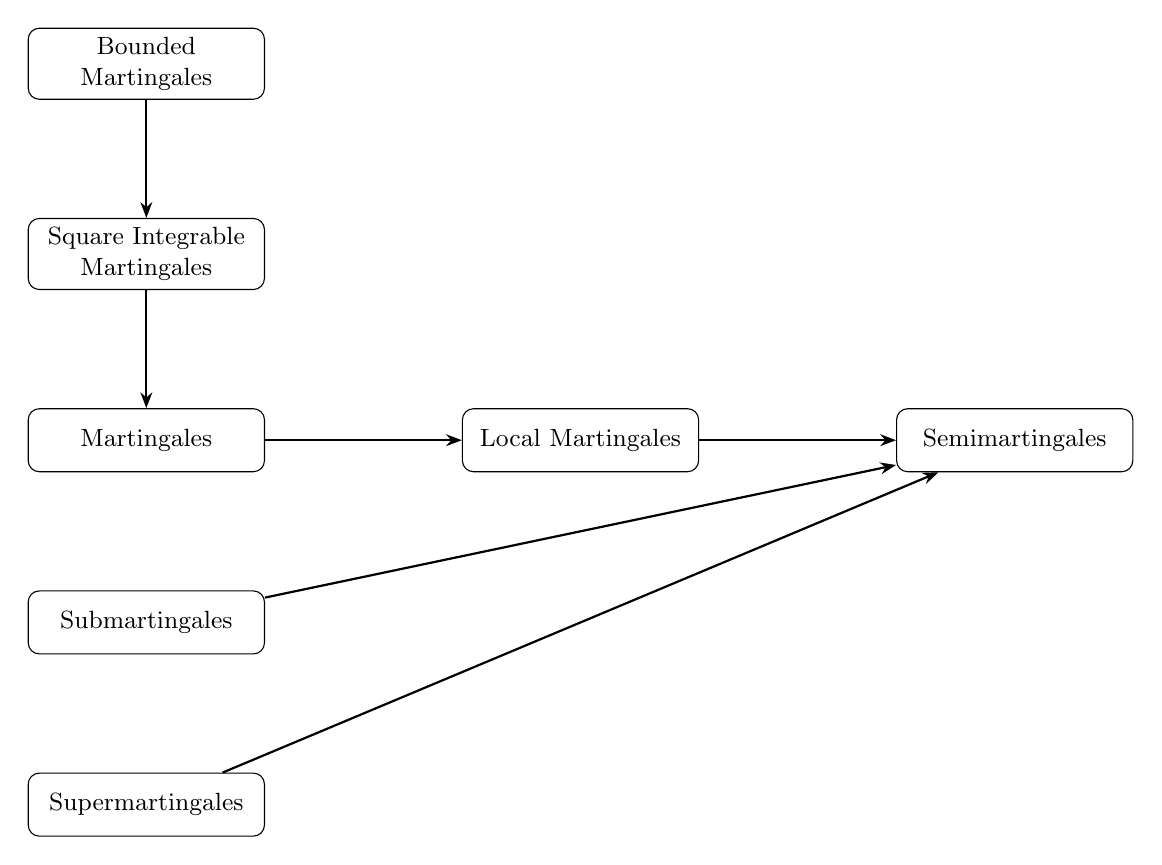
\begin{tikzpicture}[
    node distance=1.5cm and 2.5cm,
    box/.style={rectangle, draw, rounded corners, minimum width=3cm, minimum height=0.8cm, align=center, font=\small},
    arrow/.style={-{Stealth[length=2mm]}, thick}
]
    % Nodes
    \node[box] (mg) {Martingales};
    \node[box, right=of mg] (lmg) {Local Martingales};
    \node[box, right=of lmg] (smg) {Semimartingales};
    \node[box, above=of mg] (sqmg) {Square Integrable\\Martingales};
    \node[box, above=of sqmg] (bddmg) {Bounded\\Martingales};
    \node[box, below=of mg] (submg) {Submartingales};
    \node[box, below=of submg] (supmg) {Supermartingales};

    % Arrows (A -> B means A is a subclass of B)
    \draw[arrow] (bddmg) -- (sqmg);
    \draw[arrow] (sqmg) -- (mg);
    \draw[arrow] (mg) -- (lmg);
    \draw[arrow] (lmg) -- (smg);
    \draw[arrow] (submg) -- (smg);
    \draw[arrow] (supmg) -- (smg);
\end{tikzpicture}
\end{document}
